\textbf{Gamma Function} \\
\defn For $1<a\in\R$ we define
\[ \Gamma(a) = \int_0^\infty t^{a-1}e^{-t} \d t \]
\eg
\[ \Gamma(1) = \int_0^\infty e^{-t} \d t = \brack[\Big]{-e^{-t}}_0^\infty = 1 \]
Also
\begin{gather*}
\begin{aligned}
\Gamma(a) &= \int_0^\infty \underbrace{t^{a-1}}_u \underbrace{e^{-t}}_{\!\d v} \d t \\
&= \int u \d v = uv - \int v \d u \\
&= \brack[\Big]{-t^{a-1}e^{-t}}_0^\infty + \int_0^\infty (a-1)t^{a-2} e^{-t} \d t \\
&= 0 + (a-1)\int_0^\infty t^{a-2}e^{-t} \d t \\
&= (a-1)\Gamma(a-1) \qquad \text{for $a>2$} \\
\end{aligned} \\
\boxed{\Gamma(a) = (a-1)\Gamma(a-1) \qquad\text{for $a>2$}} % boxed
\end{gather*}
$\Gamma(2)=1\cdot\Gamma(1)=1$, $\Gamma(3)=2\Gamma(2)=2\cdot1$, $\Gamma(4)=3\Gamma(3)=3!$,
\begin{gather*}
\boxed{\Gamma(n+1) = n!} \\
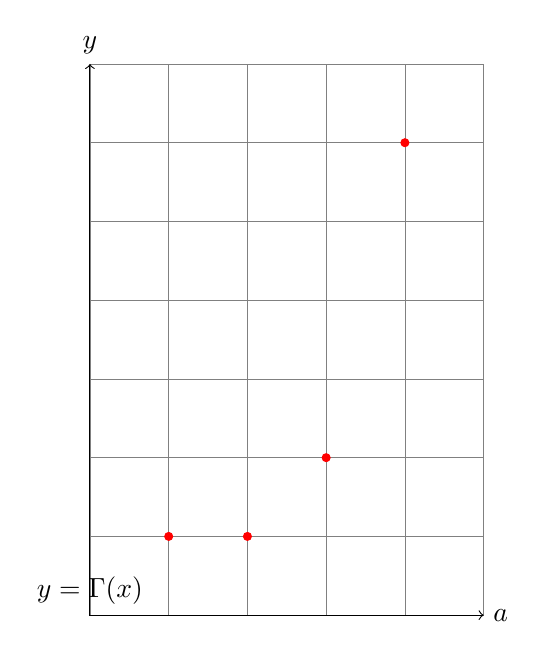
\begin{tikzpicture}[domain=0:4.1]
\draw[gray,very thin] (0,0) grid (5,7);
\draw[<->] (0,7)node[above]{$y$} -- (0,0) -- (5,0) node[right]{$a$};
\draw[<->,smooth,color=red,thick] plot[id=f] function{gamma(x)}node[above,black]{$y=\Gamma(x)$};
\draw[red,fill](1,1)circle(0.05);
\draw[red,fill](2,1)circle(0.05);
\draw[red,fill](3,2)circle(0.05);
\draw[red,fill](4,6)circle(0.05);
\end{tikzpicture}
\end{gather*}
\eg
\begin{align*}
\Gamma(\tfrac12) &= \int_0^\infty t^{-1/2}e^{-t}\d t \\
&= \int_{u=0}^\infty \frac1u e^{-u^2} 2u\d u\footnote{where $u=t^{1/2}$, $u^2=t$, $2u\d u=\!\d t$} \\
&= 2\int_0^\infty e^{-u^2}\d u
\end{align*}
Say $I=\int_0^\infty e^{-u^2}\d u$.  Then
\begin{align*}
I^2 &= \int_0^\infty e^{-x^2}\d x \int_0^\infty e^{-y^2}\d y \\
&= \int_{y=0}^\infty \int_{x=0}^\infty e^{-x^2-y^2}\d x\d y \\
&= \int_{\theta=0}^{\pi/2}\int_{r=0}^\infty e^{-r^2}r\d r\d\theta \\ \intertext{\begin{center}\myvcenter{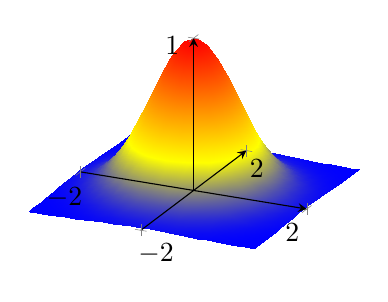
\begin{tikzpicture}
\begin{axis}[height=5cm,domain=-2:2,y domain=-2:2,z,axis lines=middle,axis on top,xtick={-2,2},ytick={-2,2},ztick={1}]
\addplot3[surf,shader=interp]{exp(-x^2-y^2)};
\end{axis}
\end{tikzpicture}}\qquad\myvcenter{\begin{tikzpicture}
\draw(0:5)arc(0:30:5)--(0,0)--cycle;
\draw(0:4)arc(0:30:4);
\node at(1,0.25){$\!\d\theta$};
\node at(4.5,-0.25){$\!\d r$};
\node at(15:5.5){$r\d\theta$};
\end{tikzpicture}}\end{center}}
&= \int_{\theta=0}^{\pi/2}\brack[\Big]{-\tfrac12e^{-r^2}}_0^\infty \d\theta \\
&= \int_0^{\pi/2}\tfrac12\d\theta = \frac\pi4 \\
\therefore I &= \int_0^\infty e^{-u^2}\d u = \frac{\sqrt\pi}{2} \\
\Gamma(\tfrac12) &= 2I = \sqrt\pi
\end{align*}
The recursion formula
\[ \Gamma(a) = (a-1)\Gamma(a-1) \]
gives
\begin{gather*}
\begin{aligned}
\Gamma(\tfrac32) &= \tfrac12\Gamma(\tfrac12) = \tfrac12\sqrt\pi \\
\Gamma(\tfrac52) &= \tfrac32\Gamma(\tfrac32) = \tfrac32\cdot\tfrac12\cdot\sqrt\pi \\
&\eqvdots \\
\Gamma(\tfrac{2n+1}{2}) &= \tfrac{2n-1}{2}\dotsm\tfrac32\cdot\tfrac12\cdot\sqrt\pi \\
%\Aboxed{ \Gamma(\tfrac{2n+1}{2}) &= \frac{(2n)!}{2^{2n}n!}\sqrt\pi }
\end{aligned} \\
\boxed{\Gamma(\tfrac{2n+1}{2}) = \frac{(2n)!}{2^{2n}n!}\sqrt\pi}
\end{gather*}
Let $U=\set{z\in\C}{\Re(z)>1}$.  For $z\in U$ we define
\[ \Gamma(z) = \int_0^\infty t^{z-1}e^{-t} \d t \]
where $t^{z-1}=e^{(z-1)\ln t}$.
\[ (\text{note that }\abs{t^{z-1}}=\abs{e^{((x-1)+iy)\ln t}}=\abs{e^{(x-1)\ln t}}=t^{x-1}) \]
This integral converges \emph{uniformly} on compact sets $K\subseteq U$. \\
\pf Let $K=[p,q]\times[r,s]$ with $p>1$.  Then
\begin{align*}
\abs[\Big]{\int_l^\infty t^{z-1}e^{-t}\d t} &\leq \int_l^\infty\abs{t^{z-1}e^{-t}}\d t \\
&= \int_l^\infty t^{x-1} e^{-t} \d t \qquad \text{where $z=x+iy$} \\
&\leq \int_l^\infty t^{q-1} e^{-t} \d t \to 0 \qquad \text{as $l\to\infty$ (independent of $z$)}
\end{align*}
since $\int_0^\infty t^{q-1}e^{-t}\d t$ converges (to $\Gamma(q)$).

It follows that $\Gamma(z)$ is holomorphic in $U$, indeed we have: \\
\thm Let $f\colon\R^+\times U\to\C$.  Suppose
\begin{enumerate}[label=\arabic*.]
\item $f$ is continuous
\item $f(t,z)$ is holomorphic in $U$ for each fixed $t\in\R^+$
\item $\int_0^\infty f(t,z)\d t$ converges uniformly in compact subsets $K\subseteq U$.
\end{enumerate}
Then the function
\[ F(z) = \int_0^\infty f(t,z) \d t \]
is holomorphic in $U$ and
\[ F'(z) = \int_0^\infty \frac{\partial}{\partial z}f(t,z) \d t . \]
\textbf{Sketch proof:} Verify that $F(z)$ is continuous.  For a triangle $\alpha$ in $U$,
\begin{align*}
\int_\alpha F(z) \d z &= \int_\alpha \int_0^\infty f(t,z) \d t\d z \\
&= \int_0^\infty \underbrace{\int_\alpha f(t,z) \d z}_{=0} \d t , \qquad \text{by Fubini's Theorem} \\
&= \int_0^\infty 0 \d t , \qquad\text{by Cauchy} \\
&= 0
\end{align*}
$\therefore F(z)$ is holomorphic in $U$ by Morera's Theorem (indeed $F(z)$ has a holomorphic antiderivative in $U$ given by
\[ G(w) = \int_\lambda F(z) \d z \]
where $a\in U$ is fixed and $\lambda$ is the line from $a$ to $w$.)
\[ \tikz{
\draw(2,1)node[right]{$z+\!\d z$}--(0,0)node[left]{$a$}--(2,0)node[right]{$z$}--cycle;
\fill(2,1)circle(1pt);
\fill(0,0)circle(1pt);
\fill(2,0)circle(1pt);
} \]
Also by Cauchy's Integral Formula, if $w\in U$ and $\sigma$ is a circle in $U$ about $w$, then
\begin{align*}
F'(w) &= \frac{1}{2\pi i} \int_\sigma \frac{F(z)}{(z-w)^2} \d z \\
&= \frac1{2\pi i} \int_\sigma \int_0^\infty \frac{f(t,z)}{(z-w)^2} \d t \d z \\
&= \int_0^\infty \underbrace{\frac1{2\pi i}\int_\sigma\frac{f(t,z)}{(z-w)^2}\d z}\d t \qquad\text{(Fubini)} \\
&= \int_0^\infty \eval{\frac{\partial}{\partial z}f(t,z)}_{z=w} \d t .
\end{align*}
\note We can use the recursion formula
\begin{align*}
\Gamma(z) &= (z-1)\Gamma(z-1) \\
&= (z-1)(z-2)\Gamma(z-2) \\
&\eqvdots \\
\Gamma(z) &= (z-1)(z-2)\dotsm(z-n)\Gamma(z-n)
\end{align*}
equivalently
\begin{gather*}
\Gamma(z+n) = (z+n-1)\dotsm(z+1)(z)\Gamma(z) \\
\mathllap{\text{\emph{or}} \qquad} \Gamma(z) = \frac{\Gamma(z+n)}{(z)(z+1)(z+2)\dotsm(z+(n-1))}
\end{gather*}
We use this to define $\Gamma(z)$ for $\Re(z)>-n+1$,
\[ z\neq0\co-1\co-2\co\dotsc\co-(n-1) . \]
Since $n\in\Z^+$ is arbitrary, we can use this to \emph{define} $\Gamma(z)$ for all $z\in\C$ except $z=0$, $-1$, $-2$, $\dotsc$ with simple poles at these points.

\thm (Euler's Reflection Formula) \\
For all $z\neq k\pi$ for $k\in\Z$,
\[ \Gamma(z)\Gamma(1-z) = \frac{\pi}{\sin \pi z} . \]
